\documentclass[a4paper,english,russian]{G2-105}
\usepackage[T1]{fontenc}
\usepackage{listings}
\usepackage{graphicx}
\usepackage{longtable}
\usepackage{booktabs}
\usepackage{standalone}
\usepackage{newclude}
\usepackage[final]{pdfpages}
\usepackage{multirow}
\usepackage{sansmath} % Enables turning on sans-serif math mode, and using other environments
\sansmath % Enable sans-serif math for rest of document
\usepackage[math]{blindtext}

%\usepackage[utf8]{luainputenc}
\VSTUSetDocumentNumbersPrefix{}
\VSTUSetDocumentCode{ВРБ-40 461 806-10.27-10-17.81}
\VSTUSetDocumentTypeDative{выпускной работе бакалавра}
\VSTUSetDocumentTypeGenitive{выпускную работу бакалавра}
\VSTUSetInitialData{задание, выданное научным руководителем с кафедры САПРиПК,
утвержденное приказом ректора}

\VSTUSetPZContents{
    \begin{VSTUList}
    \ulitem{Введение}
    \ulitem{1 Обзор технологий и фреймворков}
    \ulitem{Выводы}
    \ulitem{2 Реализация СНС с целочисленной арифметикой}
    \ulitem{Выводы}
    \ulitem{3 Оценка разработанного решения}
    \ulitem{Выводы}
    \ulitem{Заключение}
    \ulitem{Список использованных источников}
    \ulitem{Приложение A - Техническое задание}
    \end{VSTUList}
}

\VSTUSetPZGraphics{
    \begin{VSTUNumberedList}
    \ulitem{1: Название работы}
    \ulitem{2: Проблема}
    \ulitem{3: Цель и задачи}
    \ulitem{4-7: Аналоги}
    \ulitem{8: Требования}
    \ulitem{9: Проектирование. Use Case Diagram}
    \ulitem{10: Проектирование. Sequence Diagram}
    \ulitem{11-13: Реализация}
    \ulitem{14: Выводы}
    \end{VSTUNumberedList}
}


\begin{document}
\VSTUSetOrder{1548-ст}{1}{ноября}{2017}
\VSTUSetFaculty{Электроники и вычислительной техники}
\VSTUSetDepartment{Системы автоматизированного проектирования и ПК}
\VSTUSetDepartmentCode{10.27}
\VSTUSetDirection{230100 Информатика и вычислительная техника}
\VSTUSetHeadOfDepartment{и.о. зав. кафедрой САПРиПК}{д.т.н., проф.}{М. В. Щербаков}{Щербаков Максим Владимирович}
\VSTUSetDirector{доцент каф. САПРиПК}{к.т.н.}{А. В. Катаев}{Катаев Александр Вадимович}
\VSTUSetFacilityExpert{}{}{}{}
\VSTUSetStandardsAdviser{доцент каф. САПРиПК}{к.т.н.}{О. А. Шабалина}{Шабалина Ольга Аркадьевна}
\VSTUSetStudent{ИВТ-461}{Т. А. Мельников}{Мельников Тимофей Алексеевич}
\VSTUSetTitle{Портирование сверточной нейросети на ARM архитектуру с ограниченными вычислительными ресурсами и ресурсами памяти}
\VSTUSetTitleEng{Porting a convolutional neural network on an ARM architecture, taking into account the computing resources and memory resources}
%\VSTUAddChapterWordToTOC % обязательно для ПЗ в магистерских диссертациях
\VSTUInitializePZ
\abstract{Аннотация}
\par Документ представляет собой пояснительную записку к выпускной работе бакалавра на тему «Портирование сверточной нейросети на ARM архитектуру с ограниченными вычислительными ресурсами и ресурсами памяти», выполненную студентом группы ИВТ-461, Мельниковым Тимофеем Алексеевичем.
\par В данной работе рассмотрена возможность реализации алгоритмов машинного обучения, в частности прямой проход сверточной нейронной сети, на устройстве с ограниченными вычислительными ресурсами и ресурсами памяти.
\par Объём пояснительной записки составил \totalpages~страниц и включает \totalfigures~рисунков и \totaltables~таблицы. 

%\newpage
\tableofcontents
\newpage

\starchapter{Введение} \ttl
\par Задачи обработки и анализа аналоговой информации являюся одиними из самых сложных в IT-индустрии. Долгое
время такие задачи решались алгоритмами, которые требовали огромных аппаратных ресурсов при малой точности результата. На протяжении последних десяти лет стремительно растет и развивается прикладная область математики цель которой, изучение и развитие искусственных нейронных сетей \cite{1}. Актуальность разработок и исследований в данной области оправдывается применением НС в различных сферах деятельности. Это автоматизация процессов анализа объектов, образов, уневерсализация управления, прогнозирование, создание экспертных систем, анализ неформализованной информации и многое другое. В частности, в данной дипломной работе используются нейронные сети для классификации и обнаружения объектов на изображении. 
\par Наиболее существенным недостатком НС является их требовательность к вычислительным ресурсам и ресурсам памяти. Частично данная проблема решается использованием сверточных нейронных сетей, которые, в виду особенностям логики работы, позволяют в разы сократить ресурсы потребляемые нейронной сетью \cite{2}.
\par Однако, не только искусственные нейронные сети являются трендом IT-идустрии, активно развивается коцепция интернета вещей. Диапазон встраиваемых технологий простирается от концепции умных зданий до промышленной консолидации. Совмещение встраиваемых систем и искусственных нейронных сетей позволяет иначе взглянуть на решение нетревиальных задач, таких как автономное управление автомобилем \cite{3}.
\par В связи с вышесказанным целью данной дипломной работы является внедрение фреймворка машинного обучения на ARM-устройство и последующая оптимизация его работы. На основе проделанной работы необходимо сделать вывод о эффективности и рентабельности данного решения. 
\par Для достижения поставленной цели необходимо решить следующие задачи:
\begin{itemize}
\item Изучить фреймворки глубокого машинного обучения;
\item Разработать консольное приложение для реализации прямого прохода нейронной сети;
\item Оптимизировать использование оперативной памяти и реализовать загрузку весов по мере использования;
\item Разработать клиент-серверное приложение, демонстрирующее результат работы.
\end{itemize}
\par В первом разделе пояснительной записки описаны фрейворки машинного обучения. Далее приведено обоснование выбора фреймворка darknet.
\par Во втором разделе описаны используемые модели нейронных сетей и алгоритм прямого прохода.
\par Третей раздел посвящен разворачиванию фреймворка на ARM-устройсто и оптимизации работы алгоритма прямого прохода. Так же описана разработка клиент-серверной части для визуализации работы приложения. 
\newpage

\chapter{Обзор фреймворков машинного обучения} 
\par Данные раздел содержит справочную информацию, технические особенности и функциональные возможноти фреймворков глубоко машинного обучения и их сравнение. Раздел содержит обоснование выбора фреймворка Darknet для встраивания и оптимизации на мобильном пк C.H.I.P.
\par Из всего множества фрейворков были выделены Caffe, Torch7, Darknet, как наиболее зрелыe, функционально полныe и широко используемыe.
\ttl
\section{Caffe}
\par Caffe представляет собой фреймворк, разработанный учеными и практиками, с прозрачной и гибкой архитектурой для глубокого обучения и построения эталонных моделей. Фреймворк распространяется под BSD-лицензией и является c++ библиотекой. Так же реализованы python и MATLAB обертки для универсализации обучения и развертывания глубоких моделей. Caffe используется на промышленных компаниях и в медиацинтрах, обрабатывая 40 миллионов изображений в день на Titan GPU (примерно 2.5 милисекунд на изображение).
\par Caffe поддерживается и разрабатывается университетом Беркли, а именно центром BVLC.
\ttl
\subsection{Основные характеристики Caffe}
\par Caffe представляет полный набор инструментов для обучения, тестирования, настройки и разработки моделей с подробной документацией и примерами. Поэтому обучиться использовать фреймворк можно довольно быстро. Возможность использования GPU делает Caffe одним из самых быстрых фреймворков, что позволяет его использовать в промышленном секторе. Такие показатели достигнуты благодаря особенностям описаным ниже.
\par Caffe является модульным программным обеспечением. Что позволяет легко добалять новые форматы данных, слои и функции потерь. В фреймворке уже реализовано множество слоев и функций потерь, что позволяет реалзовавать нейронную сеть для задачь различных предметных областей и категорий.
\par В Caffe представление и реализация разделены. Для описания модели в Caffe используется конфигурационный файл в формате protobuf. Caffe поддерживает сетевые архитектуры в форме произвольно ориентированных ациклических графов. Важной деталей является то, что после создания экземпляра модели Caffe выделяется ровно столько памяти, сколько необходимо для работы сериализованной нейронной сети и для хранения адреса объекта \cite{4}.
\par В Caffe используется полное тестовое покрытие. Каждый модуль имеет собственный набор тестов. Модуль будет принят, только после прохождение всего набора тестов. Это позволяет эффективно оптимизировать модули и гарантирует стабильную работу фреймворка.
\par Caffe содержит предворительно обученные модели для академических целей и некоммерческого использования. Доступны сверточные НС с архитектурой "AlexNet" и вариации данной НС, обученные на базе данных ImageNet \cite{ 5}. Так же доступны реккурентные модели \cite{6}.
\ttl
\subsection{Архитектура Caffe}
\par Caffe сохраняет и передает данные в четырехмерных массивах, которые названы блобами. Блобы представляют унифицированный интерфейс для работы  памятью, содержащий пакеты ихображений (или других данных), параметров или обновлений параметров. Блобы скрывают вычислительные издержки смешанной работы CPU и GPU, выполняя синхронихацию по нере необходимости. Память выделяется по требованию (лениво), что позволяет эффективней ее использовать. Модели сохраняются как буфер, использующий протокол Google (Google Protocol Buffers), который имеет ряд достоинств: минимальный размер строки при сериализации, эффективная сериализация, высокая читабельность в текстовом виде и удобные интерфейсы работы на нескольких языках. Необходимые для обучения огромные массивы данных храняться в базах данныx LevelDB. Google Protocol Buffers и LevelDB обеспечивают пропускную способность в 150 Мб/с. 
\par Слой в Caffe представляет собой структуру соответствующую формальному определению слоя: он принимает на вход один или несколько блобов и выдает один или несколько блобов результатом. Caffe предоставляет полный набор типов слоев для глубокого обучения, включая сверточный, pooling слой, inner products слой, нелиности, такие как выпремленная линейная и логическая, слои потерь, таких как softmax и hinge. Настройка слоя требует минимальных усилий в виду композиционного построения сетей.
\par Caffe обеспечивает функциональность для любого направленного ациклического графа слоев, позволяя корректно выполнять прямой и обратный проход. Модели Caffe --- это сквозные системы машинного обученияm.
\ttl
\subsection{Приемущества Caffe}
\par От других современных фреймворков глубокого обучения Caffe отличается следующими качествами:
\begin{itemize}
	\item Реализция полностью основана на C++, что облегчает интеграцию с встраиваемыми системами. CPU режим позволяет использовать фреймворк без специализированного GPU.
	\item Готовые модели позволяют не тратить время и ресурсы на обучение. Важным пунктом является подробная документация для сериализации и использования моделей.
\end{itemize}
\ttl
\section{Torch7}
\par Torch7 --- это универсальный математический фреймворк и библиотека машинного обучения, которая имеет оболочку для языка программирования Lua. Его цель --- предоставить гибкую среду для проектирования и обучения моделей глубокого обучения. Гибкость достигается с помощью Lua, так как он является очень легким скриптовым языком. Эффективная реализация низкоуровневых числовых процедур, используя OpenMP и CUDA, позволяет фрейморку достич выской производительности. Фреймворк имеет простой Lua-интерфейс, что позволяет легко подключать его к стороннему программному обеспечению.
\ttl
\subsection{Основыне характеристики Torch7}
\par Структура фрейворка имеет три основных преимущества:
\begin{itemize}
\item она облегчает разработку численных методов;
\item фреймворк легко расширяем (включая использование сторонних библиотек);
\item высокая скорость работы фреймворка.
\end{itemize}
\par Второе преимущества достигается за счет выбранных разработчиками технологий. Скрипровый (интерпретируемый) язык с хорошим API-интерфейсом для C обеспечивает фреймворку гибкост в разработке и не накладывает ограничения на его расширяемость. Так как, язык высокого уровня делает процесс разработки программы более простым и понятным, чем язык низкого уровня. К тому же, интерпретируемость позволяет быстро и легко реализовывать различные идеи в интерактивном режиме. Хороший API-интерфейс сохраняет функциональные возможности из разных библиотек, так как становиться прослойкой между универсальной структурой на языке Lua и различными структурами используемых библиотек на языке C.
\par Высокая скорость работы достигается благодаря компилятору JIT (Just In Time). На данный момет Lua является самым быстрым интерпритируемым языком. Lua разрабатывался для легкого внедрения в приложения, написанные на C. Поэтому представляет большое C-API на основе виртуального стека, для передачи значений между Lua и C. Это унифицирует интерфейс для C/C++ и делает обертывание библиотек тривиальным.
\par Lua предназначен для использования в качестве мощного, легкого скриптового языка обладающими всеми необходимыми выразительными средствами. Он реализован как библиотека, которая написана на чистом C (точнее на подмножестве ANSI C и C++). Lua сочетает простой процедурный синтаксис с мощными конструкциями описания данных на основе ассоциативных массивов и расширяемой семантики. Lua динамически типизируется, выполняется путем интерпретации байт-кода для виртуальной машины на основе регистров и имеет автоматическое управление памятью с инкрементной сборкой мусора, что делает его идеальным для настройки, написания сценариев и быстрого прототипирования.
\par Lua предлагает хорошую поддержку объектно-ориентированного программирования, функционального программирования и программирования, управляемого данными. Основным типом Lua является таблица, которая реализует ассоциативные массивы очень эффективным способом. Ассоциативный массив --- это массив, который может индексироваться не только числами, но и любыми другими типами данных язка. Таблицы не имеют фиксированного размера, они динамически изменяемы и могут использоваться как "виртуальные таблицы" над другой таблицей, что позволяет имитировать парадигмы объектно-ориентированного программирования. Таблицы являются единственным, но очень мощным механизмом структурирования данных в Lua. Torch7 использует таблицы для простого, равномерного и эффективного представления обычных массивов, таблиц символов, кортежей, очередей и других структур данных. Lua также использует таблицы для представления пакетов \cite{7}.
\par Lua и Python очень схожи как по структурированию данных, так и по стилю программирования. Если говорить о популярности в сообществе, то Python опережает Lua из-за огромного количества поставляемых библиотек. Однако разработчики выбрали Lua по ряду других причин, которые, в виду специфики фреймворка, являются ключевыми. Во-первых, интеграция Lua с C очень проста. За несколько часов любая библиотека на C или C++ может стать библиотекой Lua. Во-вторых, Lua предоставляет эффективные возможности встраивания. Что бы преобразовать прототип в финальный продукт требуется не много дополнительной работы. В-третьих, Lua обладает высокой производительностью благорадя интерпритатору LuaJIT, который выдает производительность на уровне C. Еще одним преимуществом Lua является переносимость. Lua написан на чистом ANSI C, его можно скомпилировать для любых устройств (сотовые телефоны, встроенные процессоры в FPGA, процессоры DSP и др.) \cite{8}.
\ttl
\subsection{Структуры используемых типов данных}
\par Ключевой сущностью в Torch7 является класс Tensor, поставляемый автономной С-библиотекой Tensor. Данный класс расширяет базовый набор типов Lua, чтобы реализовать эффективную работу с многомерными массивами. Большинство пакетов Torch7 или сторонних пакетов, зависящих от Torch7, реализуют собственный класс Tensor для представления сигналов, изображений, видео и других объектов, что упрощает интегрирование различных библиотек. Библиотека Torch Tensor предоставляет множество классических операций (включая операции линейной алгебры), которые реализованны и оптимизированны на С, используются SSE интсрукции для Intel платформ. Опцианально можно использовать высокопроизовидельные реализации операций линейной алгебры в библиотеке BLAS. Так же данная библиотека поддерживает инструкции OpenMP и вычисления на CUDA GPU.
\ttl
\subsection{Пакеты Torch7}
\par На данный момент Torch7 имеет 7 основных пакетов:
\begin{itemize}
\item torch: основной пакет Torch7. Обеспечивает фреймворк классом Tensor, облегчает сереализацию и другие базовые функции;
\item lap и plot: представляют стандартные функции для создания, преобрзования и визуализации объектов Tensor. Пример работы показан на рисунке ~\ref{torch_plots}
\begin{figure}
    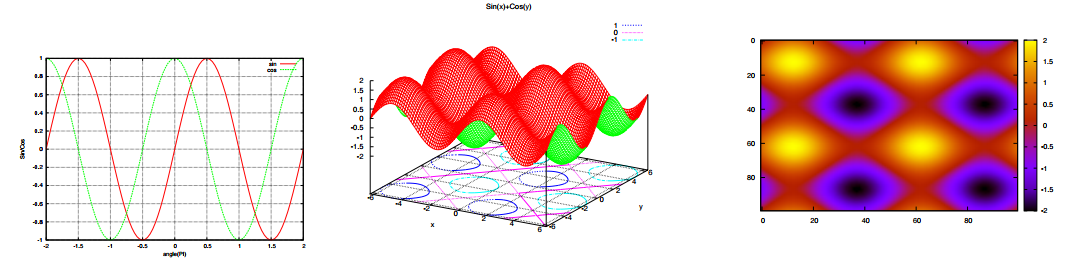
\includegraphics[width=\linewidth]{torch_plots.png}
    \caption{Графики, полученные с помощую пакета plot фреймворка Torch7. Слева: простые синусоидальные функций. В центре: Поверхность, хранящаяся в 2D Tensor. Справа: Матричный график, построенный с использованием карты тепла}
	\label{torch_plots}
\end{figure}
\item qt: предаставляет интерфейс работы Torch7 с Qt. Реализует конвертацию Tensor в QImage и наоборот. Отлично подходит для быстрого создания интерактивных демонстраци с кроссплатформенным графическим интерфейсом.
\item nn: предоставляет набод стандартных модулей для создания нейронной сети. В пакет так же входит набор контейнерных модулей, которые можно использовать для определения произвольно направленных графов. Явное описание графа позволяет избежать сложности с анализатором графов или любого другого компилятора промежуточного уровня.
\par На практике нейронная сеть представляет собой последовательные графы, либо графы с шаблонными витвлениями и рекурсиями. На рисунке ~\ref{nn_create} показано создание многослойного перцептрона, используя пакет nn.
\begin{figure}
    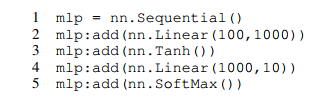
\includegraphics[width=0.3\paperheight]{nn_create.png}
    \caption{Создание многослойного перцептрона, используя пакет nn}
	\label{nn_create}
\end{figure}
\par Каждый модуль или контейнер имеет стандартные функции для вычисления выходного состояния, обратного распространения производных входов и внутренних параметров. Для нейронной сети, приведенной на рисунке ~\ref{nn_create}, вызов этих функций показан на рисунке ~\ref{nn_forward}.
\begin{figure}
    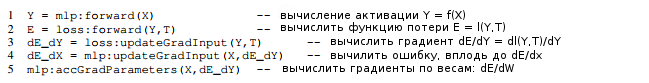
\includegraphics[width=1.2\linewidth]{nn_forward.png}
    \caption{Вычисление выходного состояния, обратного распространения производных входов и внутренних параметров}
	\label{nn_forward}
\end{figure}
\item image: пакет обработки изображений. Данный пакет поставляет стандартные функции работы с изображениями (сохранение, загрузка, маштабирование, вращение, конвертация цветовых пространст, свертка и др.).
\item optim: компактный пакет, который обеспечивает фреймворк методами оптимизации. В него входят реалиция наклонного спуска, сопряженного градиента и алгоритма Бройдена --- Флетчера --- Гольдфарба --- Шанно (BFGS).
\item unsup: содержит алгоритмы обучения без учителя, такие как K-means, разреженное кодирование и автокодеры.
\end{itemize}
\par В дополнение к основным доступен постоянно растущий список сторонних пакетов. К примеру, mattorch, который обеспечивает двухсторонний интерфейс между матричным форматом Matlab и форматом Tensor или parallel, который предоставляет функции разветвления и исполнения Lua-кода на локальных или удаленных машинах, используя механизм сериализации Torch7. Этот список постоянно растет, поскольку Lua упращаяет интерфейс любой билиотеки C.
\ttl
\section{Darknet}
Darknet является фреймворком машинного обучения с открытым исходным кодом, написанным на C и CUDA. Он прост в установке и поддерживает вычисления как на центральном процессоре, так и на графическом.
\ttl
\subsection{Основные характерискики Darknet}
\par Darknet один из немногих фреймворков машинного обучения, который не имеет обязательных зависимостей. Что позволяет быстро разворачивать его на встраиваемых системах. На ряду с встроенным функционалом, Darket поставляется с двумя опциональными зависимостями:
\begin{itemize}
\item OpenCV --- для предоставление более широкого спектра поддерживаемых форматов изображений;
\item CUDA --- для вычислений на GPU. 
\end{itemize}
\par Обе не являются обязательными для установки фреймворка.
\par Еще одним важным преимуществом фреймворка является независимость от архитектуры системы. Darknet полностью написан на C, что делает его универсальным, а его интеграцию в встраиваемы системы или в специализированное оборудование простой и понятной. 
\par В оригинальном виде фреймворк, поставляемый разработчиками, представляет консольное приложения для работы с нейронными сетями. С помощью него можно проектрировать, обучать, тестировать нейронные сети типовых топологий. В список функций так же входит визуализация модели классификации и обучение реккурентных моделей. Однако, конфигурация файлов исходных кодов спроектирована специально для предоставляения возможности компиляции необходимых модулей в библиотеку \cite{9}. Поэтому фреймворк можно встраивать как нативную библиотеку в любой пользовательский проект.
\par Важной особенностью фреймворка является оптимизация работы с памятью и с вычислительными ресурсами. Это позволяет работать с визуальными задачами даже на устройствах с ограничеммыми ресурсами памяти. Darnket имеет две эффективные реализации сверточных нейронных сетей: сети с бинарными весами и XNOR-сети. В сетях с бинарными весами фильтры аппроксимируются двоичными значениями, что приводит к экономи памяти в 32 раза. В XNOR-сетяк как фильтры, так и входные данные для сверточных слоев являются двоичными. XNOR-сети реализуют свертки, используя в основном бинарные опирации. Это приводит к ускорению сверточныз операций в 58 раз и экономии памяти в 32 раза. Данная оптимизация позволяет запускать современный нейронные сети на центральных процессорах в режиме реального времени. Если говорить о точности работы, то классификация модели AlexNet на 2.9 \% меньше у сети с бинарными весами оп сравнению с оригинальной реализацией. Метод используемый в сетях с бинарными весами и XNOR-сетех превосходит новейшие сетевые методы бинаризации (BinaryConnect и BinaryNets) на 16 \% (тест профодился на классификаю, используя модель ImageNet) \cite{10}.
\ttl
\subsection{Используемые структуры данных}
\par Ключивыми типами данных в Darknet явлюются структуры network и layer. Структура layer представляет собой объект для параметров слоя сети. Данная структура имеет общий интерфейс для всях типов слоев, поэтому обладает большим набором параметров. Для расчета выходов и градиента слоев, структура предоставляет два указателя на функции forward и backward соответственно. Реализации данных функций находятся в файлах исходных кодов у каждого типа слоя. Такая модульная структура позволяет быстро добавлять новый типы слоев и компактно реализовывать операции работы с нейронной сетью. В целом, слои представляют двунаправленный связанный список, что соответствует логике работы с нейронными сетями. 
\par Структура network определяет абстрактную модель для хранения внутренних параметров нейронной сети. Как и Caffe, Darknet разделяет представление и реализацию. Это реализуется разделением данных модели на конфигурационный файл, в котором определены внутренние параметры, и на бинарный файл с весами модели. Конфигурационный файл имеет строковый формат и представляет собой описание параметров нейронной сети, параметров обучения, параметров слоев и их последовательность. Формат конфигурационного файла представлен на рисунке ~\ref{network_cfg}
\begin{figure}
    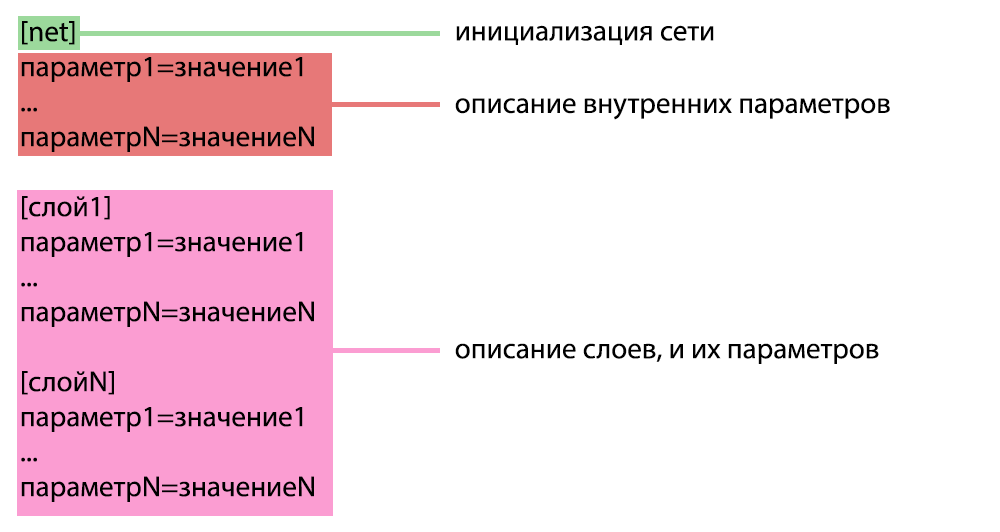
\includegraphics[width=0.4\paperheight]{network_cfg.png}
    \caption{Формат конфигурационного файла нейронной сети}
	\label{network_cfg}
\end{figure}
\par Основной структурой данных в фреймворке является динамический массив. Веса, изображения, строковые таблицы храняться в одномерном массие, который обернут в структуру соответствующего типа данных. Данный подход позволяет сократить издержки работы с памятью.
\ttl
\starsection{Выводы}
Для использования сверточной нейронной сети на системе с ограниченными вычислительными ресурсами и ресурсами памяти необходимо, что бы фреймворк, поставляющий данные функции удовлетворял следующим условиям:
\begin{itemize}
\item высокопроизворительные вычисления;
\item оптимизированная работа с памятью;
\item минимальное число зависимостей.
\end{itemize}
\par Рассмотринные выше фреймворки, используя различные терхнологии и алгоритмы, обеспечивают высокую производительность своих реализаций. Caffe использует библиотеку BLAS (ATLAS, Intel MKL, OpenBLAS) для векторных и матричных вычислений, Lua в совокупности с технологиями SSE, OpenMP позволяют Torch показывать высокую скорость работы, бинаризация ядер в Darknet, позволяет использовать быстрые бинарные операции для расчетов.
\par Если говорить о оптимизации работы с памятью, то аппроксимация фильтров и входов в Darknet позволяет значительно уменьшить объем выделяемой памяти. На рисунке ~\ref{binary_conv} сравнение бинарной свертки и свертки с двойной точностью.
\begin{figure}
    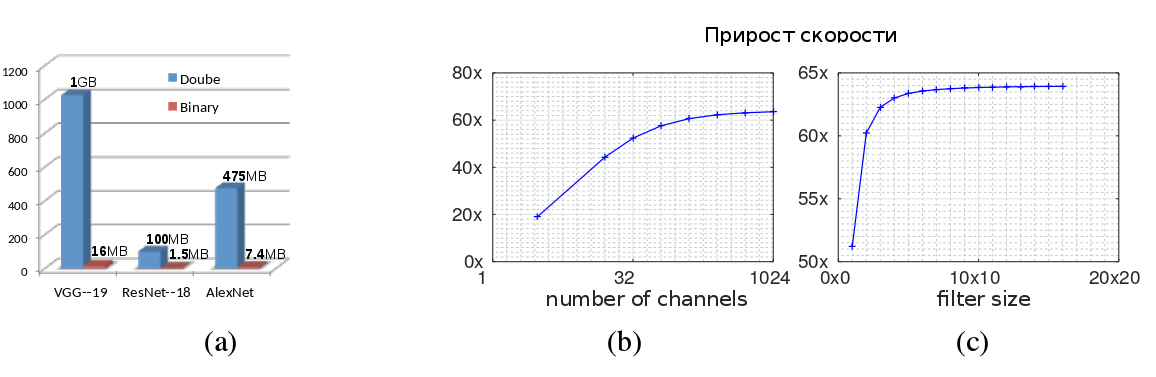
\includegraphics[width=0.55\paperheight]{binary_conv.png}
    \caption{Эффективность использования памяти и вычислений. a -- выделяемая память для весов различных архитектур, b --- ускорение в зависимости от числа каналов, c --- ускорение в зависимости от размера фильтра}
	\label{binary_conv}
\end{figure}
\par Caffe и Torch имеют достаточно большое количество зависимостей. Это объясняется желанием максимально ускорить процессы обучения и прохода нейронных сетей, однако наклабывает ограничения на срециализированное оборудование и оборудование с ограниченными запасами физической памяти.
\par Суммировав все показатели, можно сделать вывод, что Darknet является лучшим вариантов для разворачивания на маломощном ARM-устройтве.

\chapter{Используемые алгоритмы и модели}
\section{Нейронные сети: основные положения}
\par Основой любой нейронной сети являются однотипные, простые элементы, которые представляют собой упрощенную модель нейронов мозга. Далее по тексту термин “нейрон” используется для определения ячейки нейронной сети --- искусственного нейрона. В соответствии с клетками головного мозга, которые могут быть возбужденными или заторможенными, нейрон характеризуется состоянием в момент прохода нейронной сети. Каждый нейрон обладает набором синапсов и одним аксоном. Синапсы являются однонаправленными связями, которые связывают конкретный нейрон с выходами группы других нейронов. В свою очередь, аксон передает сигнал нейрона на синапсы нейронов, расположенных на следующем слое. На рисунке ~\ref{neuron} представлен общий вид нейрона. Каждый синапс описывается величиной синаптической связи, иными словами, синапсы характеризуются весом $w_i$, который является аналогом электрической проводимости в клетках мозга.
\begin{figure}
    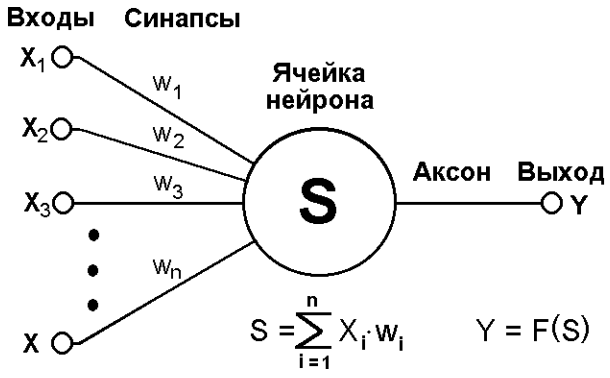
\includegraphics[width=0.6\linewidth]{neuron.png}
    \caption{Исскуственный нейрон}
	\label{neuron}
\end{figure}
\par Состояние нейрона в момент прохода нейронной сети определяется как взвешенная сумма его входов:

\[
\ \hspace*{66mm} s = \sum_{i=1}^n x_i w_i \hspace*{62mm} (1)
\] 
\par Выходом нейрона является функция от его состояния:
\[
\ \hspace*{66mm} y = f(x) \hspace*{66mm} (2)
\] 
\par Функция f должна обладать свойством нелинейности. Это необходимо для создания многослойных нейронных сетей. Если в НС используется пороговая функция, то смысла в ее многослойности нет, так как такая сеть эквивалентна сети с одним скрытым слоем и с весовой матрицей единственного слоя \cite{11}. 
\par Нелинейная функция f именуется активационной функцией нейрона. На данный момент существует огромное количество видов активационных функций. На рисунке ~\ref{activation_func} показаны некоторые из них.
\begin{figure}
    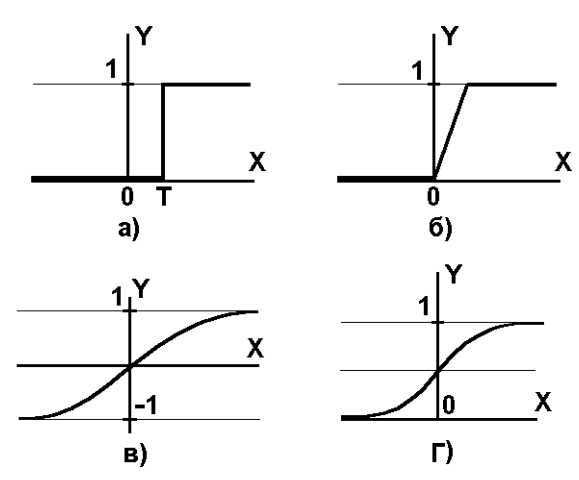
\includegraphics[width=0.6\linewidth]{activation_func.png}
    \caption{а) функция единичного скачка; б)линейный порог (гистерезис); в) сигмоид – гиперболический тангенс; г) сигмоид – формула (3)}
	\label{activation_func}
\end{figure}
\par Одной из самых первых используемых активационных функций является логистическая функция или сигмоид (функция имеет S-образный вид): 
\[
\ \hspace*{66mm} f(x) = \frac{1}{1 + e^{- \alpha x}}\ \hspace*{56mm} (2)
\] 
\par Чем меньше параметр $\alpha$, тем функция становится более пологой. В пределе при $\alpha=0$ сигмоид вырождается в горизонтальную прямую в значении 0.5. Если увеличивать a, то сигмоид преобразуется в функцию единичного скачка в точке $x=0$. Значение данной активационной функции лежит в интервале [0, 1]. Популярность функции обеспечивает простота ее производной, которая используется при обучении НС. 
\[
\ \hspace*{66mm} f'(x) = \alpha f(x) (1 - f(x)) \ \hspace*{56mm} (2)
\] 
\par Логистическая функция дифференцируема на всей оси абсцисс. Это свойство используется в некоторых алгоритмах обучения. Также, сигмоид усиливает слабые сигналы лучше, чем большие, это позволяет избежать перенасыщения от больших сигналов, так как области определения больших сигналов соответствуют пологому наклону функции.   
\par Если говорить про обработку сигналов НС, то, зачастую, они обрабатываются параллельно. Это достигается с помощью объединения большой группы нейронов в слои и соединения определенным образом нейроны разных слоев. Существуют конфигурации, где нейроны одного слоя соединены между собой. Данная конфигурация обрабатывается послойно.
\par На рис ~\ref{perceptron} изображен простейшая конфигурация нейронной сети --- трехнейронный перцептрон. Пусть нейронной этой НС используют активационную функцию в виде скачка. 
\begin{figure}
    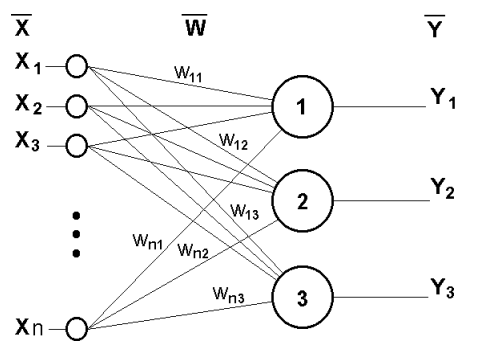
\includegraphics[width=0.4\linewidth]{perceptron.png}
    \caption{Однослойный перцептрон}
	\label{perceptron}
\end{figure}
\par На n входов поступают некоторые сигналы, которые распространяются на три нейрона, образующие скрытый слой НС. Каждый нейрон выдает сигнал:
\[
\ \hspace*{66mm} y_j = f\biggl[\sum_{i=1}^n x_i w_{ij} \biggr], j=1 \dots 3  \ \hspace*{56mm} (2)
\] 
\par Из весовых коэффициентов можно составить матрицу W, в которой wij -- вес i-того входного сигнала в j-том нейроне. Тогда, процесс прохода НС описывается в матричной форме следующим образом:
\[
\ \hspace*{66mm} Y=F(XW)  \ \hspace*{56mm} (2)
\] 
где X --- вектор входных сигналов, Y --- вектор выходных сигналов, F(XW) --- активационная функция, выполняющаяся над каждым элементом вектора XW \cite{12}.
\par Теоретически количество слоев (глубина) и количество нейронов в них (высота), используемых в НС, не ограниченно, но фактически ограничения накладывают вычислительные мощности устройства, на котором выполняется обработка НС. Но чем сложнее НС, тем масштабнее задачи она может решить. 
\par Структура НС зависит от сложности задачи. Оптимальные конфигурации для некоторых типов задачи уже реализованны и описаны, например в \cite{13}. Если же задача не является типовой, то разработчик самостоятельно генерирует модель, в зависимости от сложности задачи, размера обучающей выборки и вычислительных ресурсов. При этом необходимо учитывать основопологающие принципы: качество модели напрямую зависит от количества нейронов сети, плотности связей между ними и количеством слоев; сложность алгоритмов функционирование сети (например, введение нескольких типов синапрос, использование непороговых активационных функций) влиет на производительность НС. Задача поиска оптимальной конфигурации для той или иной задачи является отдельным направлением нейрокомпьютерной науки. Синтез нейронной сети напряму зависит от типа решаемой задачи, поэтому список подробных рекомендаций составить затруднительно. В большинстве случаев оптимальный вариант выбирается эмпирическим методом.
\par Очевидно, что функционирование нейронной сети напрямую зависит от величины синаптических связей между нейронами. Поэтому, после нахождения конфигурации нейронной сети, разработчик должен найти оптимальные значения всех переменных весовых коэффициентов (некоторые веса могут быть постоянными).
\par Описанный процесс называется обучений нейронной сети, он является ключевым при сознании НС. От того, насколько хорошо он будет выполнен, зависит качество решений поставленных задачь перед нейронных сетей. На этапе обучение кроме качества поиска весов важное место занимает такой параметр как время обучения. Эти два параметра обратно пропорциональны: чем лучше подобраны веса, тем больше затрачено времени на обучение.
\par Сущетвует два варианта обучения: с учителем и без него. В первом случае, при обучении предоставляются как входны сигналы, так и желаемые выходные. Далее обучение представляет собой алгоритм подгонки весов, таким образом, что бы желаемы выходные сигнали совпадали с выходными сигналами НС. Во втором случае, выходы генерируется нейронной сетью, а при обучении учитываются только входные и производные от них сигналы.
\par Существующие алгоритмы машинного обучения делятся на два типа: детерминистские и стохастические. В первом случае подбор оптимальных весом представляет собой четкую последовательность, во втором --- подчинен некоторому случайному процессу. 
\par Необходимо сказать, что среди классификаций НС важное место занимают бинарные и аналоговые сети. Первые используют двоичные сигналы, в результате чего выход каждого из нейров принимает одно из двух значений: логический ноль ("заторможенное" состояние) или логическая единица ("возбужденное" состояние). К такой классификации относится перцептрон, описанные выше. Его активационная функция является пороговой, значение которой либо 0 либо 1. В аналоговых сетях выходное значение нейронов может быть непрерывным, это реализуется использованием в качестве активационных непрерывные функции, например сигмоид. 
\par Еще одна классификация разделяет НС на синхронные и асинхронные. Первый случай предпологает изменение состояния только одного нейрона в каждый момент времени. Во втором случае изменние произходит одновременно у группы нейронов, как правило, у всего слоя. Ход времени в НС представлен последовательным выполненим однотипных действий над нейронами. В данной главе будут рассмотрены только синхронные НС.
\par Обычно, сети классифицируют по числу слоев. На ~\ref{perceptron2} показана НС полученная добавлением еще одного слоя, состоящего из двух нейронов, в НС, изображенную на ~\ref{perceptron}. Слои, которые не являются входными и выходными, называются скрытыми. 
\begin{figure}
    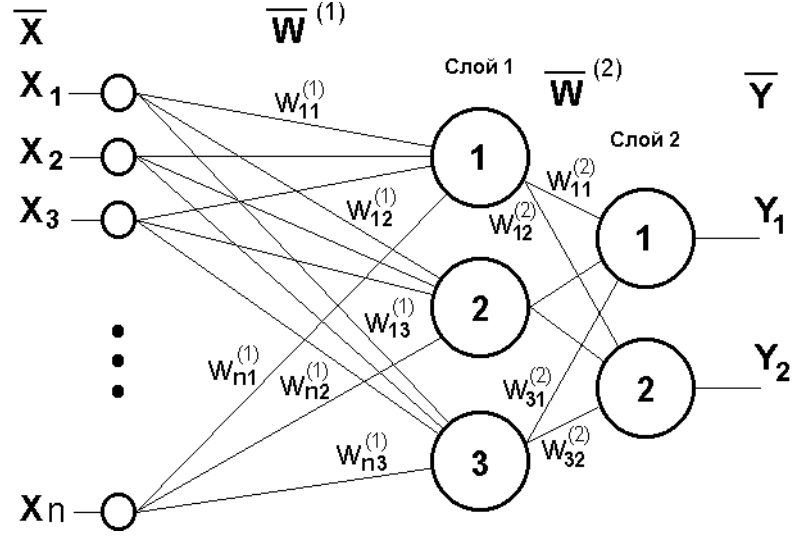
\includegraphics[width=0.6\linewidth]{perceptron2.png}
    \caption{Двухслойный перцептрон}
	\label{perceptron2}
\end{figure} 
\par Бывают случае, когда нелинейность используется еще и в синаптических связях. Большинство современных сетей используют формулу (1) для вычисления значения нейронна, однако, для эффективного решения некоторых задач используется другая запись, например:
\[
\ \hspace*{66mm} s = \sum_{i=1}^n x_{i}^{2} w_i  \ \hspace*{56mm} (2)
\] 
\par или даже
\[
\ \hspace*{66mm} s = \sum_{i=1}^n x_{i}^{2} x_{((i+1)\bmod n)} w_i  \ \hspace*{56mm} (2)
\] 
\par Главное, что бы разработчик понимал, какие цели он преследует при наделении нейрона подобной связью и какие ограничения на нейрон накладываются. Введение таких нелинейность увеличивает вычислительную мощность НС, другими словами, позволяет уменьшить число нейронов и связей без потери качества работы[8]. 
\par При обучении НС учитывается не только время процесса и качество обучения. Помимо этих параметров необходимо подобрать пороговое значение T. Из рисунка ~\ref{activation_func} видно, что, в общем случает, T может принимать произвольное значение. То же самое относиться и к центральной точке сигмоиды, положение которой изменяется по оси X влево или вправо. В общем случии каждая активационная функция имеет параметр, который необходимо подобрать при обучении. В связи с этим формула (1) должа выглядеть следующим образом:
\[
\ \hspace*{66mm} s = \sum_{i=1}^n x_{i} w_i-T \ \hspace*{56mm} (11)
\] 
\par Что бы добавить данное смещение, необходимо добавить еще один вход, которые меет синаптическую связь со всеми нейронами слоя. На этот вход всегда "возбужденный" сигнал. Присвоим такому входу номер 0. Тогда
\[
\ \hspace*{66mm} s = \sum_{i=1}^n x_{i} w_i-T \ \hspace*{56mm} (11)
\] 
\par где $w_0=-T, x_0=1.$
\par Из чего следует, что отличие формулы (1) от формулы (12) в способе нумерации входов.
\par Все задачи, которая решает НС можно свести к классификации. Грубо говоря задача НС обпределить к какому классу принадлежит группа входных сигналов, находящихся в n-мерном пространстве. С математической точки зрения процесс представляет собой разбиение гиперпространство гиперплоскостями на области.
\par К каждой области принадлежит отдельный класс. Максимальное число классов для НС перцептронного типа не превышает $2^m$, где m --- число выходов сети. Однако существует ограничение на формы гиперплоскостей, иначе говоря, не все нейронные сети могут разделить n-мерное пространство на необходимое количество классов.
\par Например, однослойный перцептрон, с одним нейроном, изображенный на рисунке ~\ref{single_neuron} не способен разделить двумерное пространство на две
полуплоскости так, что бы классифисировать входные сигналы на классы A и B (см. ~\ref{a_and_b}).
\begin{figure}
    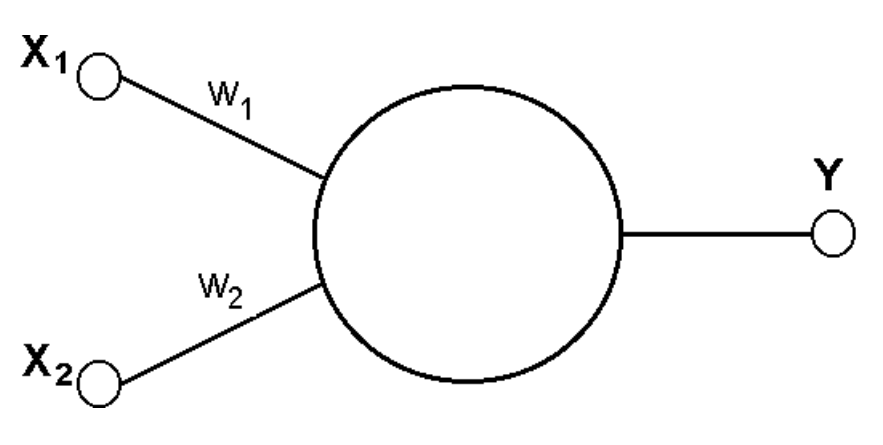
\includegraphics[width=0.6\linewidth]{single_neuron.png}
    \caption{Однонейронный перцептрон}
	\label{single_neuron}
\end{figure}
\begin{longtable}{|c|c|c|c|}
    \caption{Классификация XOR}\\ \hline
    \label{a_and_b} 
    x1 & x2 & A & B \\ \hline
    0  & 0  & • & \hspace*{1mm}  \\ \hline
    0  & 1  & \hspace*{1mm} &  • \\ \hline
    1  & 0  & \hspace*{1mm} &  • \\ \hline
    1  & 1  & • & \hspace*{1mm} \\ \hline
\end{longtable}

\par Сеть, представленная на рисунке ~\ref{single_neuron} описывает следующие уравнение:
\[
\ \hspace*{66mm} x_1 w_1 + x_2 w_2=T \ \hspace*{56mm} (11)
\] 
\par Данное уравнение является прямой, которая не способна разделить плоскольсть таким образом, что бы группа входных сигналов $x_1, x_2$ пренадлежали необходимым классам. На рисунке ~\ref{line_class} показана работа НС.
\begin{figure}
    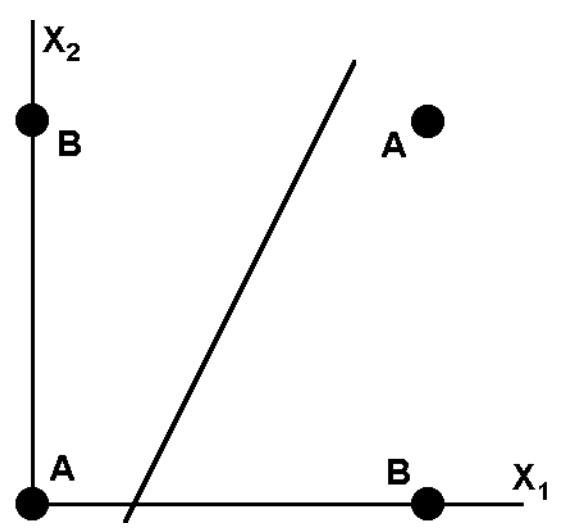
\includegraphics[width=0.6\linewidth]{line_class.png}
    \caption{Визуальное представление работы НС с рисунка ~\ref{single_neuron}}
	\label{line_class}
\end{figure}
\par Таблица ~\ref{a_and_b} является таблицей истинности для логической функции исключающего ИЛИ. Невозможность реализовать данную функцию, используя однонейронный перцептрон, получила название проблемы исключающего ИЛИ.
\par Задачи, которые не решаются однослойной сеть, называются линейно неразделимыми \cite{13}. Для решения таких задачь используются нейронные сети сбольшим количеством скрытый слоев. Однако, и в таких случаях корректное разделение на классы не гарантируется. Как было сказано раньше, конфигурация НС это итеративный эмпирический процесс.
\par После обзора теоритических основ нейроной сети, можно более подробродно рассмотреть алгоритм обучения с учителем, на основу взят перцептрон, изображенный на рисунке ~\ref{perceptron}.
\par Алгоритм выглядит следующим образом:
\par 1) Проинициализировать весовые коэффициэны случайными значениями.
\par 2) Подать на вход вектор вхожных сигналов, вычислить выходные сигналы.
\par 3) Если выход совпарает с желаемыми значениями, перейти на шаг 4.
Иначе вычислить разницу желаемым и полученным значение НС:
\[
\ \hspace*{66mm} \delta=Y_I-Y \ \hspace*{56mm} (11)
\] 
\par Изменить веса в соответствии с формулой:
\[
\ \hspace*{66mm} w_{ij}(t+1)=w_{ij}(t)+\nu        \delta x_i \ \hspace*{56mm} (11)
\]
гдe $t$ и $t+1$ --- номера текущей и следующей итерации; $\nu$ --- коэффициент скорости обучения; $i$ --- номер входа; $j$ --- номер нейрона в слое.
\par Веса будут увеличины, если $Y_I>I$, тем самым ошибка уменьшится. В обратном случае они будут уменьшены, и Y соответственно тоже уменьшится, приближаясь к $Y_I$.
\par 4) Повтор шага 2, пока не будет достигнута желаемая точность.
\par На втором шаге на вход НС подаются все входные вектора из обучающей выборки в случайном порядке. Число итераций зависит от сложности задачи и конфигурации нейронной сети. Определить точное количество итераций, необходимых для корректного обучения определить невозвожно \cite{14}. 
\ttl
\section{Сверточные нейронные сети}
\par Сверточные нейронные сети имеют схожие характеристики с обычными нейронными сетями. Они состоят из нейронов, которые имеют обучаемые веса. Каждый нейрон преобразует входные данные в выходной сигнал, который, возможно, будет изменен нелинейностью. Каждая такая сеть имеет функцию потерь на последнем полносвязным слоем.
\par Изменения заключаются в том, что архитектура сверточных сетей построена на явном предположении, что входной слой представляет собой изображения. Это предположение вносит особые свойства в архитектуру сети. Функция прямого прохода становится более эффективной для реализации и значительно уменьшаются количество параметров сети.
\par Проблема регулярных нейронных сетей заключается в невозможности маштабирования. Например, в CIFAR-10 изображения имеют размер 32x32x3 (3 цветовых канала), поэтому каждый полносвязный нейрон в первом скрытом слое будет иметь 32 * 32 * 3 = 3072 веса. Данное количество весов является приемлемым для нейронной сети, но полносвязная структура не маштобируется. Например, если на вход подается изображение с размером 200x200x3, то каждый полносвязный нейрон будет иметь 200 * 200 * 3 = 120000 весов. Поэтому посносвязная структура сети использует огромные вычислительные ресурсы и ресурсы памяти. Большое количество параметров быстро приведет к переобучению.
\par В сверточных нейронных сетях учитывается тот факт, что на вход подается изображение, поэтому архитектура таких сетей оптимальней использует ресурсы памяти. В частности, в отличие от обычных сетей, сверточные используют нейроны, имеющие 3 измерения: ширина, высота, глубина (в CIFAR-10 ширина --- 32, высота --- 32, глубина --- 3). Нейроны в слое подключены только к малой области предыдущего слоя. На изображении ~\ref{convnn} показана структура сверточной нейронной сети. Красный слой на изображении представляет входной слой. Его ширина и высота будут размером изображения, а глубина равна 3-м.
\begin{figure}
    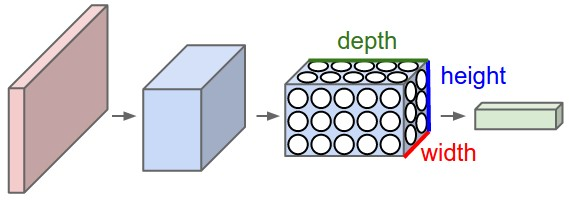
\includegraphics[width=\linewidth]{convnn.png}
    \caption{Структура сверточной нейронной сети}
	\label{convnn}
\end{figure}
\par Для построение архитектуры сверточной нейронной сети используются 3 основных типа своев: сверточный (convolution), слой объединения (pooling) и полносвязный \cite{15}. 
\par Для решение задачи классификации на размеченной базе CIFAR-10 может использоваться следующая архитектура:
\begin{itemize}
\item Вход [32x32x3]. Содержит исходные значения пикселей изображения.
\item Сверточный слой [32x32x12]. Вычисляет выходы нейронов, которые подключены к локальным областям на входе. Каждый нейрон имеет на выходе значение, вычесленное для небольшой области изображения. Это приводит к увеличению размерности слоя. В данном случае, слой будет иметь 12 фильтров, поэтому глубина слоя увеличится по отношению к входному слою.
\item RELU-слой. Проводит активацию сверточного слоя. В таком слое применяется пороговая функция активации. В нашем случает используется функция $max(0, x)$. Размер слое остается неизменным.
\item Объдиняющий слой [16x16x12]. Выполняет операцию понижения дискретизации по пространственным измерениям (ширина, высота). Такое преобразование приводит к умешьшению размерности пространственных плоскостей.
\item Полносвязный слой [1x1x10]. Вычисляет оценки классов. Наждый из 10 значений соответствуют оценке класса, среди категорий CIFAR-10. Как и в случае с обычными нейронными сетями, каждый нейрон этого слоя связан со всеми нейроннами предыдущего слоя.
\end{itemize}
\par Таким образом сверточная нейронная сеть преобразует исходные значение пикселей изображения в итоговые оценки классов. В такой сети, некоторые слои содержат параметры, а другие нет. В частности, сверточный и полносвязный слой выполняют преобразования, которые являются функцией не только активации входного сигнала, но и параметров (веса, смещения нейронов). Объединяющий и RELU слои реализуют фиксированную функцию. 
\par В итоге, можно сделать следующие выводы:
\begin{itemize}
\item Архитектура сверточной нейронной сети в простейшем случае представляет собой список слоев, которые преобразуют изображения в выходные сигланы (например, вероятности классов изображений).
\item Существуют несколько разлизных типов слоев (Сверточный, объединяющий, RELU и полносвязный являются самыми популярными).
\item Каждый слой принивает 3-x мерный массив сигналов и преобразует его в выходной 3-х мерный массив сигналов через дифференцируемую функцию.
\item Каждый слой может иметь или не иметь параметров.
\end{itemize}
\par На рисунке ~\ref{convnet} показан результат работы сверточной нейронной сети. На данном изображении визуализированны выделенные признаки нейронной сетью на каждом из этапов прямго прохода.
\begin{figure}
    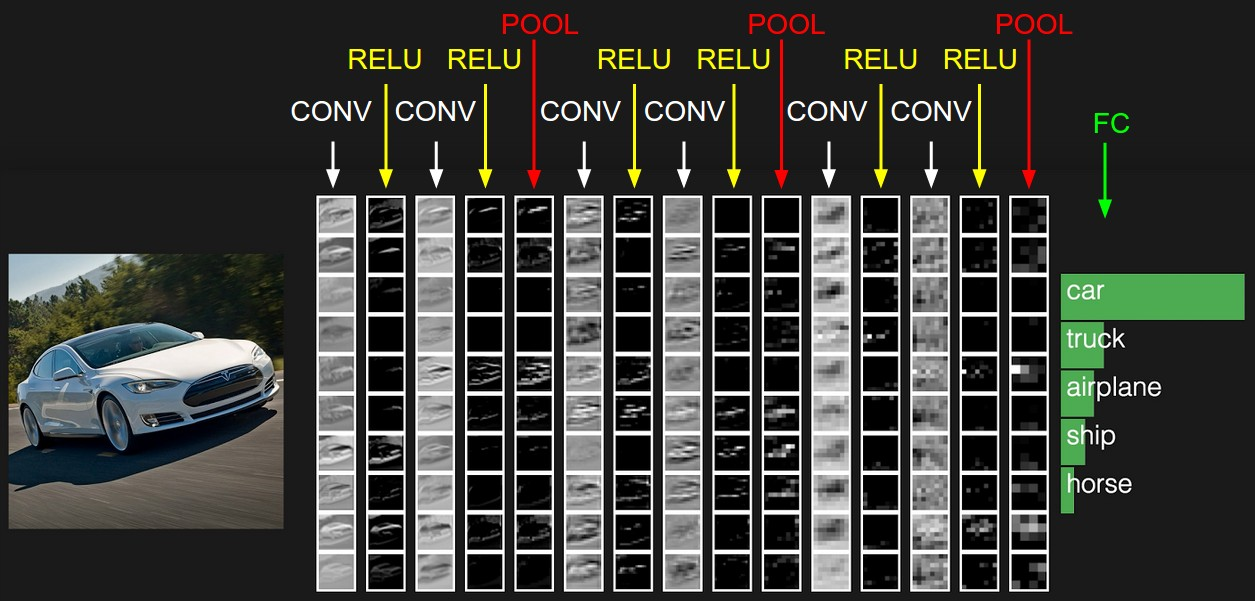
\includegraphics[width=\linewidth]{convnet.png}
    \caption{Визуализация работы сверточной нейронной сети}
	\label{convnet}
\end{figure}
\par Сверточный слой является основным стоительным блоком сверточной нейронной сети. На него затрачивается основная часть вычислительных ресурсов.
\par Для начала разберем сверточный слой без привязки к биологическому нейрону. Параметры слоя состоят из набора обучаемых фильтров. Фильтр является малым относительно входного пространства (по ширине и высоте), однако он проходит через всю глубину входного объема. Например, стандартный фильтр для первого сверточного слоя имеет размер 5х5х3 (Ширина и высота по 5 пикселей). Во время прямого прохода мы перемещаем фильтр по входному пространству и вычисляем свертку между локальными значениями входного пространства и значениями фильтра. При этом вычисляется двумерная карта активации, которая генерирует выход в каждом пространственном положении. На протяжении этого процесса сеть, активирует функции, которые представляют собой какую-либо визуальную информации. От различный линий на первом слое, и конкретные объекты изображения на конечном слое. В итоге, нейронная сеть, представленная выше, будет иметь 12 фильтров, каждый из который сгенерирует двумерную карту активаций.
\par При работе с высокоразмерными входами, такими как изображение, как было показано выше, не целесообразно связывать нейроны текущего слоя со всеми нейронами предыдущего слоя. Вместого этого в сверточных нейронных сетях каждый нейрон подключается только к локальной области входного объема. Пространственная протяженность этой связности является гирерпараметром, которые называется восприимчивым полем нейрона (размер фильтра). Важной особенносью является то, что соединения нейронов локальны в пространстве (по ширине и высоте), но всегда полны по всей глубине входного объема.
\par Например, если входным слоем является изображение 32x32x3 и размер фильра равен 5x5, то каждый нейрон в сверточном слое будет имет размер 5x5x3. В общей сложности 5*5*3 = 75 весов (и параметр смещения). 
\par На рисунке ~\ref{depthcol} показано пространственное подключение нейрона, но по полной глубине \cite{16}. 
\begin{figure}
    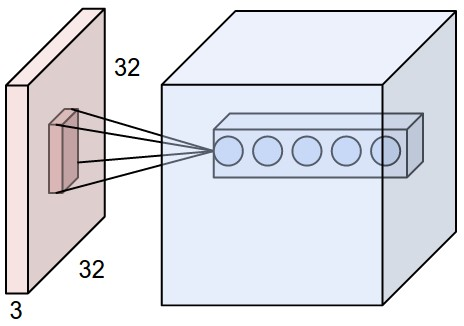
\includegraphics[width=0.5\linewidth]{depthcol.png}
    \caption{Визуализация свертчного слоя}
	\label{depthcol}
\end{figure}
\par Следующие параметры управляют размером выхода сверточного слоя:
\begin{itemize}
\item Глубина --- гиперпараметр, соответствующий числу фильтров. Каждый из фильтров обучается на поиск конкретного признака объекта.
\item Шаг --- величина на которорую сдвигается фильтр.
\item Нулевое заполнение --- размер размещений нулей вокруг границ входного пространства.
\end{itemize}
\ttl
\section{Обнаружение объектов с применем подхода YOLO}
\subsection{Преимущества YOLO}
\par Люди смотрят на изображение и сразу узнают, какие объекты находятся на изображении, где они находятся, и как они взаимодействуют. Человеческая визуальная система является быстрой и точной, что позволяет нам выполнять сложные задачи, такие как вождение автомобиля. Быстрые и точные алгоритмы обнаружения объектов позволят компьютерам управлять автомобилями без специальных датчиков. Такие алгоритмы используются для передачи вспомогательным устройствам информации о событиях в реальном времени, что расширяет потенциял для универсальных, гибких роботизированных систем.
\par На данный момент, системы обнаружения перепрофилируют классификаторы. Чтобы обнаружить объект, эти системы использют классификатор для этого объекта и оценивают его работу в различных местах изображения и в различных маштабах. Такие системы используют подход скользящего окна, где классификатор запускается в равномернорасположеных точках по всему изображению.
\par Основная идея подхода YOLO стоиться на том, что обнаружение объекта определяется как проблема с одной регрессией, от пикселов изображения до координат ограничительной рамки и вероятностей классов. Такой подход позволяет за один проход сети определить, акие объекты присутствуют на изображении и где они находятся.
\par Архитектура YOLO представляет собой сверточную нейронную сеть, которая одновременно предсказывает локализацию объекта и класс найденного объекта. На рисунке ~\ref{yolo} показана схема работы детекции. Такая модель имеет несколько преимуществ над существующими решениями детекции объектов \cite{17}.
\begin{figure}
    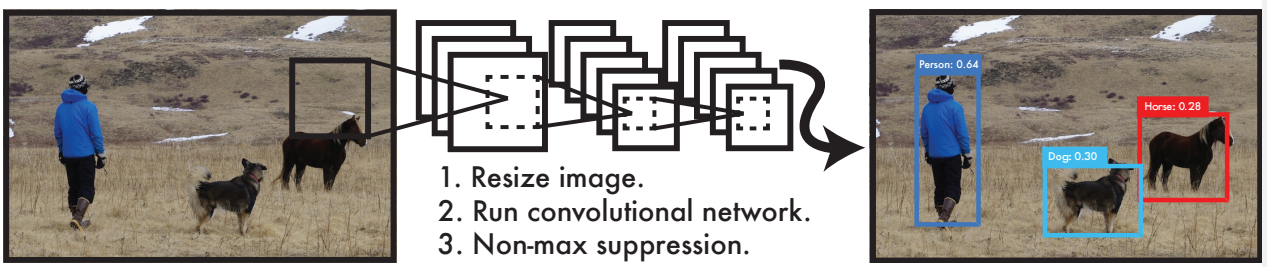
\includegraphics[width=\linewidth]{yolo.png}
    \caption{Система обнаружения YOLO}
	\label{yolo}
\end{figure}
\par Во-первых, нейронная сеть YOLO является очень быстрой. Посколько детекция расскатривается как проблема регрессии, не нужен сложный конвейвер. Кроме того, YOLO превосходит более чем в два раза среднюю точность обнаружения по сравнению с другими системами реального времени.
\par Во-вторых, YOLO учитывает весь контекст изображения. В отличии от методов, основанных на использовании окон и регионов, YOLO при обучении учитывает не только конкретный объект, но и контекстуальную информацию, которая существенно влияет на точность детекции. 
\par В-третьих, YOLO обобщает предсавления объектов. При обучении на естественных изображениях и тестировании на художественных работах YOLO превосходит методы детекции, такие как DPM и R-CNN.
\subsection{Алгоритм единого обнаружения}
\par Сеть YOLO делит входное изображение на сетку $SxS$. Если центр объекта попадает в ячейку сетки, эта ячейка сетки отвечает за обнаружение этого объекта.
\par Каждая ячейка сетки предсказывает $B$ ограничивающих рамок и оценки доверия для этих рамок. Эти оценки доверия отражают уверенность модели в том, что в рамке содержится объект. Формально, величина доверия определяется следующим образом:
\[
\ \hspace*{66mm} Pr(Object)*IOU_{pred}^{truth},  \ \hspace*{56mm} (11)
\]
\par где $Pr$ --- функция определяющая величину вероятности объекта, $IOU_{pred}^{truth}$ --- метрика пересечения между предсказанной локализацией и дейтвительным местоположением объекта.
\par Если объекта нет в данной ячейке, то оценка доверия должна быть равна нулю. В обратном случае, величина доверия равна пересечению между предстказанным местоположением и действительным местоположением объекта.
\par Каждый ограничивающий блок состоит из 5 прогнозов: $x, y, w, h$ и величина доверия. Координаты $(x, y)$ представляют собой центр блока относительно границ ячейки сетки. Ширина и высота предсказываются относительно всего изображения. Величина доверия представляет собой $IOU$ между предсказанным блоком и дейтвительным местоположением объекта.
\par Каждая ячейка сетки также пресказывает вероятности условного класса $C$. Эти вероятности обусловлены ячейкой сетки, содержащей объект \cite{18}.
\begin{figure}
    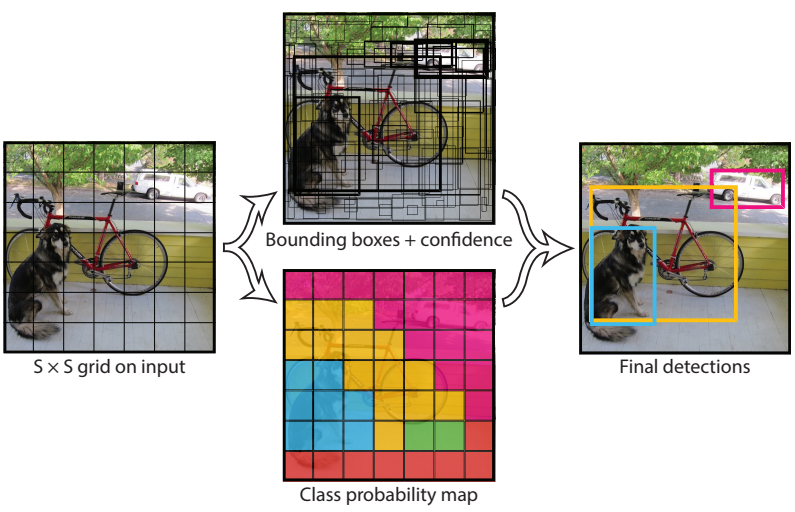
\includegraphics[width=0.7\linewidth]{yoloiter.png}
    \caption{Модель YOLO}
	\label{yoloiter}
\end{figure} 
\par Во время тестирования условные вероятности классов и идивидуальные оценки доверия каждого блока. Эта оценка интерпритируется как вероятность того, что данный класс имеется в блоке и насколько предсказанный блок подходит для данного объекта. 

\par Суммировав вышесказанное, алгоритм работы YOLO выглядит следующим образом:
\begin{itemize}
\item Разделение изображения на сетку $SxS$;
\item Предсказание ограничивающих блоков $B$;
\item Предсказание классов $C$ для объектов в каждом блоке.
\end{itemize}
\par На рисукне ~\ref{yoloiter} изображена визуальная модель сети YOLO.
\ttl
\starsection{Выводы}
\par Сверточные нейронные сети являются наиболее оптимальным вариантом для решение задачи детектирования изображений на маломощном устройстве. Это обусловлено спецификой архитектуры данного типа нейронных сетей. Сверточные и объединяющие слои позволяют троекратно сократить затраты вычислений и оперативной памяти при прямом проходе за счет уменьшения размерности признаков.
\par Сверточной сети YOLO позволяют реализовать алгоритм детектирование объектов с минимальными затратами вычислительных ресурсов. Важным приемуществом данного подхода является целостность архитектуры. При использовании YOLO достаточно один раз совершить прямой проход сети по изображению, что бы детектировать объекты на нем, что значительно уменьшает количество вычислений по сравнению с методами сколзящего окна \cite{19}.
\chapter{Проектирование системы}
\section{Архитектура системы}
\par Для полноценного функционирования система разделена на две части: клиентскую и серверную.
\par Клиентское приложение запускается на персональном компьютере и имеет GUI-интерфейс для общения c пользователем. В свою очередь серверное приложение, запускаемое на ARM-устройстве выполняет детекцию изображения и возвращает результат клиентскому приложению в виде размеченного изображения. Взаимодействие между клиенстким и серверным приложением осуществляется посредством TCP-сокетов.
\ttl
\subsection{Проектирование клиентского приложения}
\par Клиенское приложение необходимо для демонстрации вычислений сверточной нейронной сети, которая производится на ARM-устройстве. Оно представляет собой GUI-интерфейс, в котором пользователю предоставлются следующие возможности:
\begin{itemize}
\item Подключение к серверному приложению на ARM-устройстве;
\item Выбор изображения для детекции;
\item Запуск детекции на сервере;
\item Просмотр информации о этапах работы сервера;
\item Завершение работы серверного приложения.
\end{itemize}
\par На рисунке ~\ref{usecase} показана диаграмма вариантов использования клиенского приложения.
\par Что бы получать информацию о выполненных этапах детекции изображения на сервере, запущен дополнительный поток, который ожидает сообщения от сервера и выводит сообщение в текстовый браузер. 
\par В приложении 2 технического задания изображена диаграмма последовательности, на которой показана какая информация поступает от серверного приложения и в какой последовательности. 
\begin{figure}
    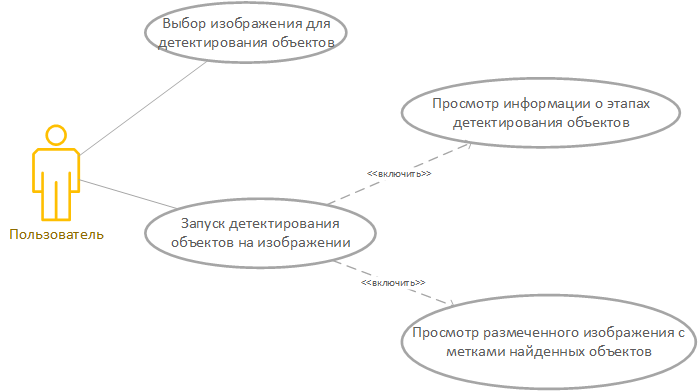
\includegraphics[scale = 0.7]{usecaseclient.png}
    \caption{Диаграмма вариантов использования клиенского приложения}
	\label{usecase}
\end{figure}
\ttl
\subsection{Проектирование серверного приложения}
\par Серверное приложение выполняется на ARM-устройстве. Оно реализует взаимодействие с клиентской частью, используя сокеты, и детекцию объектов на изображении с использованием API фреймворка darknet.
\par После подключения клиента, серверное приложения ожидает команды от клиентского приложения. Для запуска детекции изображения используетса команда "yolo". На рисунке ~\ref{state} изображена диаграмма деятельности, на которой показны функции, выполняемые серверным приложением в зависимости от поступившей команды клиетского приложения.
\par Завершение работы серверного приложение происходит при получении команды "exit". При этом серверное приложение закрывает дискриптор сокета, через который совершался обмен сообщениями.
\par Для обмена сообщениями между клиентским и серверным приложением реализован общий интерфейс передачи данных. В него входят функции приема и отправки текстовых сообщений и изображений.
\begin{figure}
    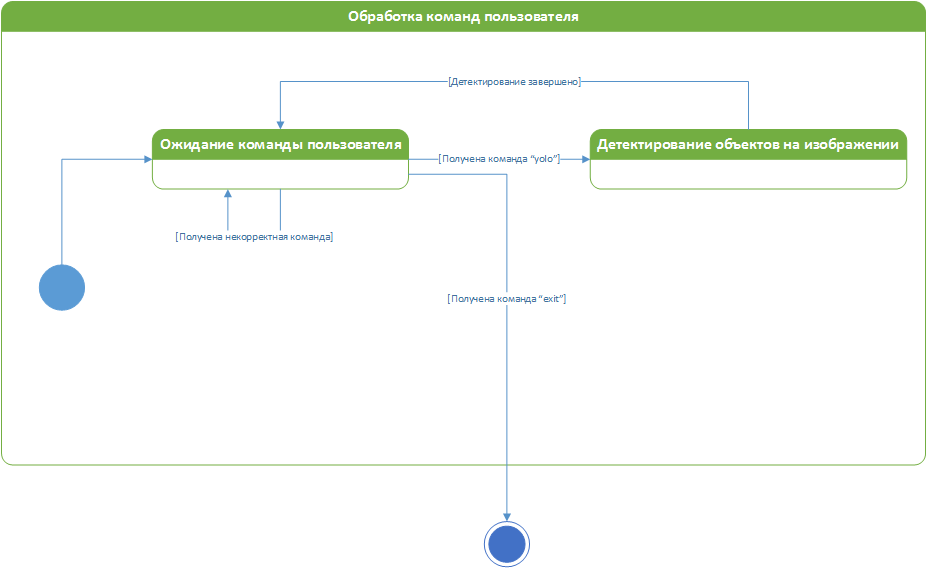
\includegraphics[width=\linewidth]{statediagramserver.png}
    \caption{Диаграмма деятельности серверного приложения}
	\label{state}
\end{figure}
\ttl
\subsection{Проектирование алгоритма прямого прохода сверточной нейронной сети}
\par Для реализации детектирование объектов на изображении используется API фреймворка darknet. В время работы детекции изображения серверное приложение отсылает клиенту информацию о пройденых этапах детекции. На рисунке ~\ref{activitydetector} изображена диаграмма последовательности, на которой показаны этапы детекции.
\par Для реализации прямого прохода нейронной сети использовались следующие функции, реализованные в фреймворке darknet:
\begin{itemize}
\item read\_data\_cfg --- осуществляет парсинг меток классов;
\item parse\_network\_cfg --- осуществляет парсинг конфигурации нейронной сети;
\item load\_weights --- сериализует веса нейронной сети;
\item load\_image\_color --- сериализует изображение для детекции;
\item network\_predict --- осуществляет прямой проход сериализованной нейронной сети;
\item draw\_detections --- осуществляет отрисовку ограничивающих объекты блоков и меток объектов.
\end{itemize}
\begin{figure}
    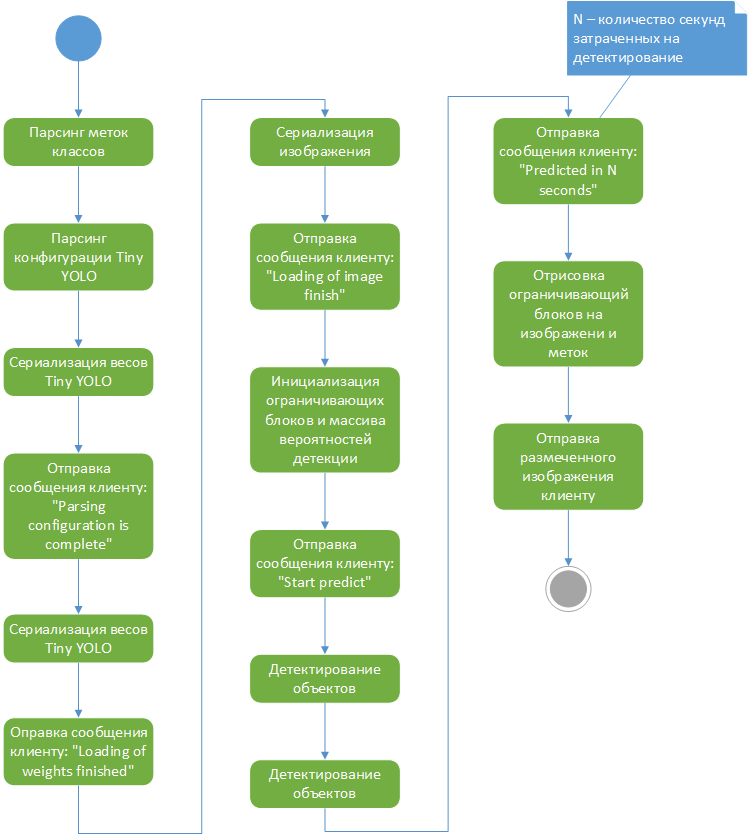
\includegraphics[width=0.8\linewidth]{activitydetector.png}
    \caption{Диаграмма последовательности алгоритма детектирования объектов}
	\label{activitydetector}
\end{figure}
\ttl
\section{Особенности реализации прямого прохода сверточной нейронной сети}
\par Для уменьшения затрат оперативной памяти при прямом проходе сверточной нейронной сети были произведены следущие мероприятия:
\begin{itemize}
\item Для реализации прямого прохода использовалась сверточная нейронная сеть Tiny YOLO;
\item После прохождения очередного слоя, память затраченная на его сереализацию очищается.
\end{itemize}
\par Архитектура сверточной нейронной сети Tiny YOLO в два раза меньше оригинальной сети YOLO. Соответсвенно занимаемая память на хранение сети уменьшилась в два раза. В приложении Б изображена архитектура Tiny YOLO. В таблице ~\ref{mbtable} показано количество занимаемой памяти сетью Tiny YOLO.
\begin{longtable}{|c|c|c|}
    \caption{Количество памяти, необходимое для сериализации весов Tiny YOLO} \label{mbtable} \\ \hline
    Имя слоя        & Размер слоя        &    Необходимое количество памяти, Мб \\ \hline \endhead
    Data           & 448x448x3 & 2,408 448 \\ \hline
    Conv1           & 224x224x64 & 12,845 056 \\ \hline
    Pool1           & 112x112x64 & 3,211 264 \\ \hline
    Conv2           & 112x112x192 & 9,633 792 \\ \hline
    Pool2           & 56x56x192 & 2,408 448 \\ \hline
    Conv3           & 56x56x128 & 1,605 632 \\ \hline
    Conv4           & 56x56x256 & 3,211 264 \\ \hline
    Conv5           & 56x56x256 & 3,211 264 \\ \hline
    Conv6           & 56x56x512 & 6,442 528 \\ \hline
    Conv7           & 28x28x256 & 0,802 816 \\ \hline
    Conv8           & 28x28x512 & 6,442 528 \\ \hline
    Conv9           & 28x28x256 & 0,802 816 \\ \hline
    Conv10           & 28x28x256 & 0,802 816 \\ \hline
    Conv11           & 28x28x256 & 0,802 816 \\ \hline
    Conv12           & 28x28x512 & 6,442 528 \\ \hline
    Conv13           & 28x28x256 & 0,802 816 \\ \hline
    Conv14           & 28x28x512 & 6,442 528 \\ \hline
    Conv15           & 28x28x512 & 6,442 528 \\ \hline
    Conv16           & 28x28x1024 & 3,211 264 \\ \hline
    Fc17           & 1x1x4096 & 0,016 384 \\ \hline
    Fc19           & 1x1x1470 & 0,005 880 \\
\end{longtable}
\par Суммарное количество памяти, необходимо для сериализации Tiny YOLO составляет 79,601 Мб. Это является приемлемыми затратами для мобильного пк C.H.I.P., который использользовался как ARM-устройство в данной работе. Однако, при прямом проходе каждого сверточного и объединяющего слоя генерируюся выходные сигналы. Поэтому, ресурсов C.H.I.P. не достаточно для осуществления прямого прохода. 
\par Для того, что бы оптимизировать работу с оперативной памятью при выгрузке слоев, был видоизменена функция прямого прохода нейрнных сетей в фрейворке darnket. Сам фремворк интегрируется посредством компилирования исходных файлов фреймворка в исполняемый файл серверного приложения. На рисунке ~\ref{alg} показаны различия между оригинальным алгоритмом прямого прохода и видоизмененным.
\begin{figure}
    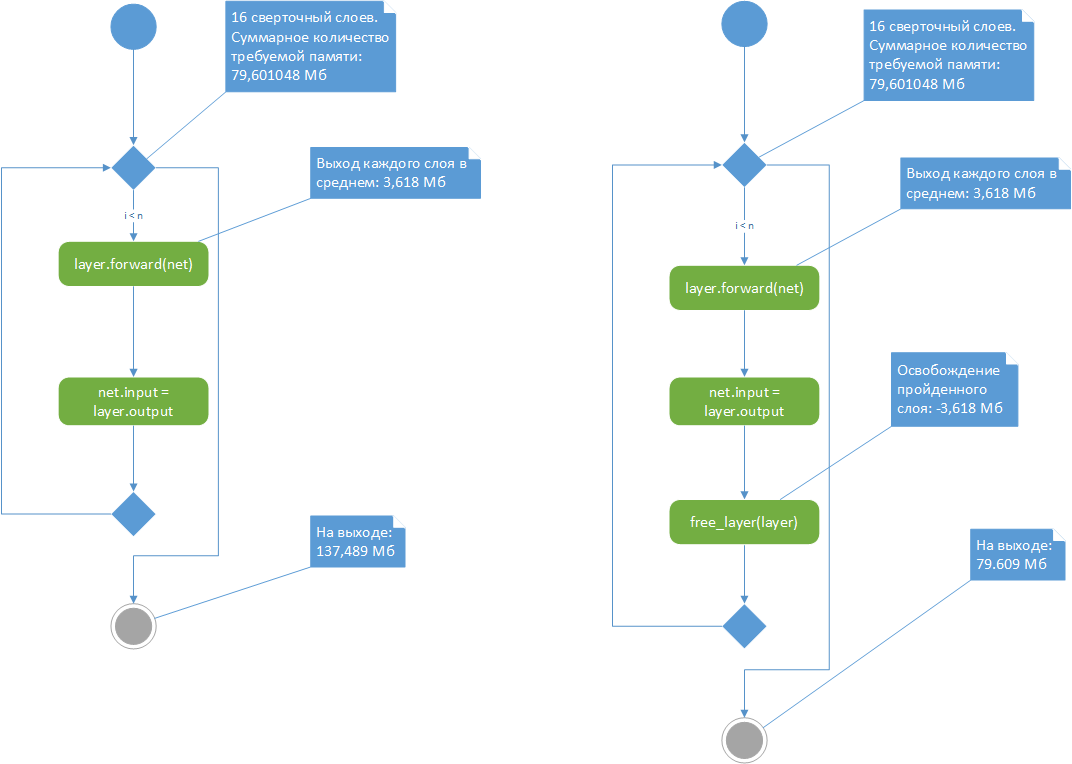
\includegraphics[width=\linewidth]{alg.png}
    \caption{Различие между оригинальным алгоритмом прямого прохода и видоизмененным}
	\label{alg}
\end{figure}
\par Удаление слоя после его прохода, позволяет уменьшать затраты оперативной памяти на каждой итераци вычислений и позволяет осуществлять детектирование объектов на маломощном устройстве C.H.I.P.
\ttl
\section{Требования к входным/выходным данным приложения}
\par Входными данными для клиентского приложения является изображения в форматах png и jpg.
\par Входными данными для серверного приложения являются файл с метками объектов, на детекцию которых обучена нейронная сеть формата data, конфигурационный файл формата cfg, изображение для детектирования в форматах png и jpg, веса нейронной сети в формате weights. В приложении 1 технического задания описаны форматы конфигурационных файлов нейронной сети.
\par Выходными данными системы является изображение с отображением меток детектированного изображения, данные о этапах детектирования и время выполнения детектирования.
\par На рисунке ~\ref{window} показан результат работы детектирования изображения. Слева на изображении отмечены прямоугольником обнаруженные объекты. Справа отображена информация об основных этапах детектирования данного изображения.
\begin{figure}
    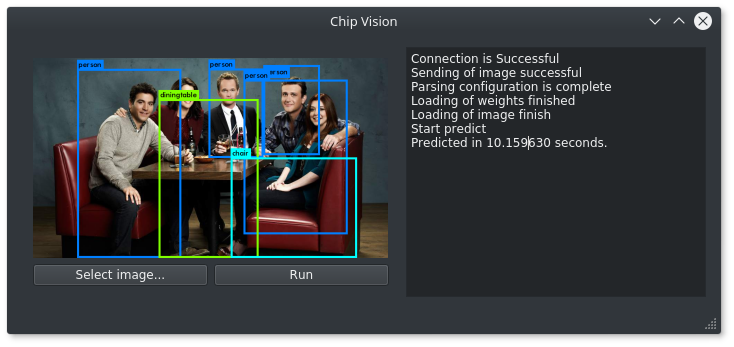
\includegraphics[width=\linewidth]{window.png}
    \caption{Пример работы детекции объектов}
	\label{window}
\end{figure}
\ttl
\section{Тестирование разработанного приложения}
\par На рисунке ~\ref{timedetection} показно время на детектирование изображений различных разрешений.
\begin{figure}
    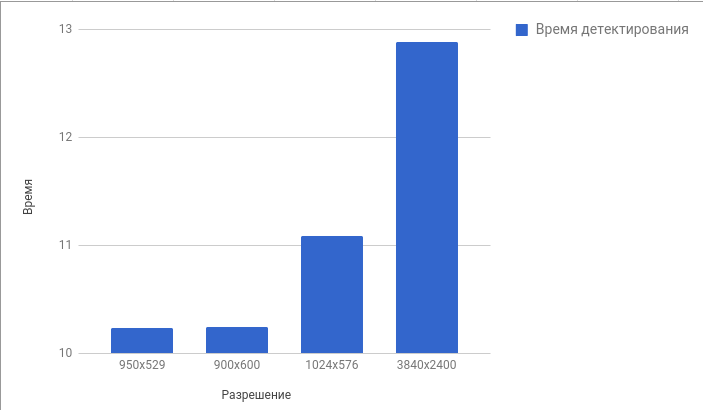
\includegraphics[width=0.6\linewidth]{timedetection.png}
    \caption{Диаграмма зависимости времени детекции от разрешения изображения}
	\label{timedetection}
\end{figure}
\par В среднем время на детектирование объектов состовляет 10,5 минут. С увеличением размерности изображение время увеличивается, это связано с затратами на изменение размера изображения.
\newpage
\starchapter{Заключение}
\par На основании проделанной рабоыт можно сделать следующие выводы:
\begin{itemize}
\item Были проанализированны фреймворки глубинного машинного обучения;
\item Были проанализированны подходы к детекции объектов на изображении;
\item Разработан алгоритм детектирования объектов на изображении для маломощного ARM-устройства;
\item Программно реализованно серверное приложение, выполняющее детектирование объектов на маломощном ARM-устройстве;
\item Программно реализованно клиентское приложение, которое демонстратирует результаты работы серверного приложения.
\end{itemize}
\par Разработанная система позволяет сделать вывод о возможности реализации систем машинного обучения на маломощных устройствах. Однако, для реализации требовательных к вычислительным ресурсам и ресурсам памяти алгоритмов машинного необходимо выполнять следущие ограничения:
\begin{itemize}
\item использование алгоритмов и архитектур с наименьшим количеством геперпараметров;
\item оптимиированная работа с памятью;
\item отсутствие зависимостей.
\end{itemize}
\newpage
\begin{thebibliography}{1}
	\bibitem{1} A Quick Introduction to Neural Networks [Electronic resource]. --- Mode of access : https://ujjwalkarn.me/2016/08/09/quick-intro-neural-networks/ (date of access 12.03.2017).
	\bibitem{2} Advantages and disadvantages of using artificial neural networks [Electronic resource]. --- Mode of access : http://www.sciencedirect.com/science/article/pii/S0895435696000029 (date of access 12.03.2017).
	\bibitem{3} The Advantages of an Embedded System [Electronic resource]. --- Mode of access : https://www.techwalla.com/articles/the-advantages-of-an-embedded-system (date of access 12.03.2017).
    \bibitem{4} Caffe: Convolutional Architecture for Fast Feature Embedding [Electronic resource]. --- Mode of access : https://arxiv.org/pdf/1408.5093.pdf (date of access 21.05.2017).
    \bibitem{5} ImageNet classification with deep convolutional neural networks [Electronic resource]. – Mode of access : https://www.nvidia.cn/content/tesla/pdf/machine-learning/imagenet-classification-with-deep-convolutional-nn.pdf (date of access 25.05.2017).
    \bibitem{6} Decaf: A deep convolutional activation feature for generic visual recognition [Electronic resource]. – Mode of access : http://proceedings.mlr.press/v32/donahue14.pdf (date of access 25.05.2017).
    \bibitem{7} Torch7: A Matlab-like Environment for Machine Learning [Electronic resource]. –  Mode of access : https://www.nvidia.cn/content/tesla/pdf/machine-learning/imagenet-classification-with-deep-convolutional-nn.pdf (date of access 27.05.2017).
    \bibitem{8} Справочное руководство по языку Lua 5.1 [Электронный ресурс]. – Режим доступа : http://www.lua.ru/doc/1.html (дата обращения 23.05.2017).
    \bibitem{9} Darknet: Open Source Neural Networks in C [Electronic resource].
— Mode of access : https://pjreddie.com/darknet/ (date of access 22.03.2017).
    \bibitem{10} XNOR-Net: ImageNet Classification Using Binary Convolutional Neural Networks [Electronic resource]. – Mode of access : https://pjreddie.com/media/files/papers/xnor.pdf (date of access 30.05.2017).
    \bibitem{11} Монахова, Е. Д. "Нейрохирурги" с Ордынки / Е. Д. Монахова // PC Week/RE. – 2013. – № 9. --- С 25-28.
    \bibitem{12} Уоссермен, Ф. Нейрокомпьютерная техника: Теория и практика / Ф. Уоссермен ; перевод Зуев Ю. А., Точенов В. А. – Москва : Мир, 1992. – 184 c.
    \bibitem{13} Итоги науки и техники. Серия Физические и математические модели баз данных и нейронных сетей / Российская акад. наук, Всероссийский ин-т науч. и технической информ. – Москва : ВИНИТИ, 2007. – 351 c.
	\bibitem{14} Нейронная сеть – введение [Электронный ресурс]. – Режим доступа : http://robocraft.ru/blog/algorithm/558.html (дата обращения
28.05.2017).
    \bibitem{15} Neural Network Architectures — Mode of access :
https://medium.com/towards-data-science/neural-network-architectures-156e5
(date of access 11.04.2017)
    \bibitem{16} Deep Learning with Limited Numerical Precision / Suyog Gupta
[etc.] // ICML’15 Proceedings of the 32nd International Conference on
International Conference on Machine Learning : Lille, France, July 06-11,
2015. / International Conference on Machine Learning. — Lille, France, 2015. —  Volume 37. — Pages 1737-1746.
    \bibitem{17} YOLO: Real-Time Object Detection [Electronic resource]. – Mode
of access : https://pjreddie.com/darknet/yolo/ (date of access 16.04.2017).
    \bibitem{18} You Only Look Once: Unified, Real-Time Object Detection [Electronic resource]. – Mode of access : https://pjreddie.com/media/files/papers/yolo\_1.pdf (date of access 11.05.2017).
    \bibitem{19} YOLO9000: Better, Faster, Stronger [Electronic resource]. – Mode of access : https://pjreddie.com/media/files/papers/YOLO9000.pdf (date of access 17.05.2017). 
\end{thebibliography}
\appendixdocument{Техническое задание}
\appendix{Архитектура сверточной нейронной сети Tiny YOLO}
\begin{figure}
    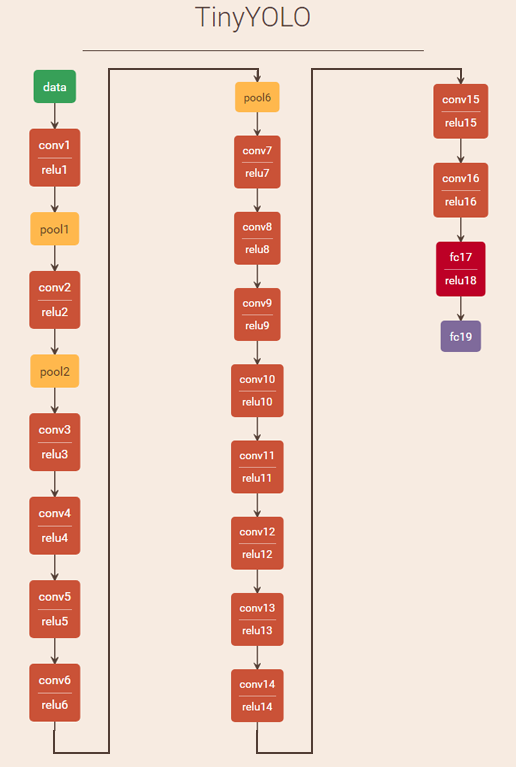
\includegraphics[width=0.75\linewidth]{tinyyoloar.png}
    \caption{Конфигурация сверточной нейронной сети Tiny YOLO}
	\label{tinyyoloar}
\end{figure}
\end{document}
